%% Compile: latexmk -pdf main.tex
\documentclass[11pt]{article}

\usepackage[a4paper,margin=2.6cm]{geometry}
\usepackage{amsmath,amssymb,amsthm}
\usepackage{booktabs}
\usepackage{graphicx}
\usepackage{microtype}
\usepackage{lmodern}
\usepackage[T1]{fontenc}
\usepackage[utf8]{inputenc}
\usepackage[round]{natbib}
\usepackage[colorlinks=true,linkcolor=blue,citecolor=blue,urlcolor=blue]{hyperref}

\newtheorem{proposition}{Proposition}
\newtheorem{remark}{Remark}

\newcommand{\bz}{\mathbf{z}}
\newcommand{\bmu}{\boldsymbol{\mu}}
\newcommand{\E}{\mathcal{E}}
\newcommand{\Hent}{\mathcal{H}}

\title{Free Energy Is a Signed, Zero-Training Detector of Acquisition Shift
in Frozen Vision--Language Encoders:\\
A Pre-Registered Falsification Study on Medical Image Corruptions}

\author{Houssem Eddine Lassoued\\
\small University Research Laboratory, Tunis, Tunisia\\
\small \texttt{houssem.lassoued@example.edu}}

\date{September 1, 2026 (revised September 5, 2026)}

\begin{document}
\maketitle

\begin{abstract}
Frozen vision--language encoders such as CLIP enable zero-shot medical image
classification in which class anchors are text embeddings and the softmax
posterior over image--anchor distances is exactly a Gibbs distribution at
temperature $T=2\tau$, where $\tau$ is the temperature learned during
contrastive pre-training. This identification makes two label-free observables
available at no training cost: the Shannon entropy $\Hent$ of the posterior and
the Helmholtz free energy $F$ of the underlying energy model. Because a uniform
translation of the anchor distances leaves $\Hent$ invariant but shifts $F$, we
pre-registered a falsifiable prediction: under increasing acquisition shift,
$F$ separates source from corrupted images
($\mathrm{AUROC}\!\ge\!0.70$) while $\Hent$ stays near chance
($\mathrm{AUROC}\!\le\!0.60$). We tested this prediction with a strictly
zero-training protocol---prompts frozen before any target evaluation,
temperature fixed at $2\tau$, every reported number traceable to a versioned
run---on the official MedMNIST-C corruptions of BreastMNIST (ultrasound, seven
corruptions) and PneumoniaMNIST (chest X-ray, four corruptions), with paired
DeLong tests and stratified bootstrap confidence intervals. The strong form of
the prediction is \emph{refuted}: entropy is never near chance. What the data
reveal instead is sharper. On structural corruptions (pixelation, JPEG, motion
blur, speckle) $F$ dominates $\Hent$ significantly (severity-5 AUROC up to
$1.000$ vs.\ $0.888$; paired $\Delta$AUROC $+0.080$ to $+0.208$, all
$p<0.05$), whereas photometric corruptions (brightness, contrast, X-ray
Gaussian noise) \emph{decrease} $F$ and drive the one-sided detector below or
near chance (AUROC $0.127$--$0.594$): free energy is a \emph{signed} shift score.
A two-sided variant $|F-\mathrm{med}_{\mathrm{source}}(F)|$, calibrated on
source images only, restores above-chance detection on five of six
sign-inverted cases (e.g., $0.127\!\to\!0.803$) while preserving the structural
ones. Across prompt reformulations $F$ is markedly more stable than $\Hent$
(severity-5 AUROC dispersion $0.03$ vs.\ $0.08$). All code, per-run metrics and
raw scores are released; refuted criteria are reported as pre-registered.
\end{abstract}

\section{Introduction}
\label{sec:intro}

Zero-shot classification with frozen vision--language encoders
\citep{radford2021clip} is an attractive substrate for medical imaging:
class definitions are text prompts, no gradient touches the backbone, and the
deployment surface is a single forward pass. Yet clinical images arrive from
scanners, probes and acquisition protocols that drift over time and across
sites, and a deployed zero-shot pipeline needs a label-free signal that the
input distribution has moved \citep{rabanser2019failing}. Such a signal is the
gating quantity for every downstream mechanism studied in test-time adaptation
(TTA) \citep{wang2021tent,shu2022tpt,yoon2024ctpt,niu2022eata,niu2023sar}:
whether to adapt, when to stop, and which samples to refer to a human reader.

This paper studies the cheapest conceivable such signal. When image embeddings
$\bz$ are scored against $K$ fixed text anchors $\bmu_k$, the CLIP posterior is
a Gibbs (Boltzmann) distribution over squared distances at temperature
$T=2\tau$ (Section~\ref{sec:theory}). Two observables then come for free: the
prediction entropy $\Hent$---the workhorse of TTA objectives and confidence
baselines \citep{hendrycks2017msp,wang2021tent}---and the Helmholtz free
energy $F$, the log-partition function popularized for out-of-distribution
detection on classifier logits \citep{liu2020energy,grathwohl2020jem,lecun2006ebm}
and later transposed to vision--language models \citep{ming2022delving}.

Our starting point is a structural asymmetry between the two. If an
acquisition shift moves images away from \emph{all} anchors roughly uniformly
--- adding a constant $c$ to every energy $E_k$ --- the posterior and hence
$\Hent$ are unchanged, but $F$ shifts by exactly $c$. This motivated a
\emph{pre-registered, falsifiable} prediction (criteria fixed before any
target data were scored, Section~\ref{sec:protocol}): under increasing
corruption severity, $F$ detects the shift
($\mathrm{AUROC}\ge 0.70$) while $\Hent$ remains near chance
($\mathrm{AUROC}\le 0.60$), with a margin of at least $0.05$.

We tested this prediction under a deliberately austere protocol: no training,
no adaptation, prompts frozen \emph{a priori} and published verbatim,
temperature fixed at the theoretical value $2\tau$, and every number in this
paper generated by a versioned script and stored in a per-run metrics file.
The testbed is MedMNIST-C \citep{disalvo2025medmnistc}, the corruption
benchmark built on MedMNIST~v2 \citep{yang2023medmnist}, on two modalities:
breast ultrasound (BreastMNIST, derived from BUSI
\citep{aldhabyani2020busi}) and chest X-ray (PneumoniaMNIST, derived from
\citealp{kermany2018pneumonia}).

\paragraph{Findings.} The strong form of the prediction is \emph{refuted}:
$\Hent$ is never near chance (severity-5 AUROC $0.462$--$0.888$), because
realistic corruptions do not translate energies uniformly. The refutation,
however, uncovers a structure that we believe is more useful than the original
conjecture:

\begin{enumerate}
\item \textbf{A structural/photometric dichotomy.} On corruptions that destroy
spatial structure (pixelation, JPEG compression, motion blur, speckle noise),
$F$ dominates $\Hent$ significantly as a shift detector. On photometric
corruptions (brightness, contrast, X-ray Gaussian noise), corrupted embeddings
move \emph{closer} to the text anchors, $F$ decreases, and the one-sided
detector drops below chance --- to $0.127$ in the worst case. Free energy is a
\emph{signed} score, not a magnitude.
\item \textbf{A source-calibrated two-sided rescue.} The statistic
$|F - \mathrm{med}_{\mathrm{src}}(F)|$, using only the source median, restores
above-chance detection on five of the six sign-inverted cases while leaving
structural detection essentially intact.
\item \textbf{Prompt stability.} Across three prompt reformulations, the
severity-5 detection AUROC of $F$ varies by $\sim$$0.03$ while that of
$\Hent$ varies by $\sim$$0.08$: the partition function is more robust to the
wording that defines the anchors than the posterior shape is.
\end{enumerate}

We report the pre-registered verdict in full, including the criteria that
failed, and release code, metrics and raw scores for every run.

\section{Theoretical framework}
\label{sec:theory}

\subsection{Gibbs posterior over textual anchors}

Let $\bz\in\mathbb{R}^d$ be an $\ell_2$-normalized image embedding and
$\bmu_1,\dots,\bmu_K$ the $\ell_2$-normalized text embeddings of the class
prompts. Define the configuration energy
\begin{equation}
E_k(\bz) \;=\; \lVert \bz - \bmu_k \rVert_2^2 \;=\; 2 - 2\langle \bz, \bmu_k\rangle .
\label{eq:energy}
\end{equation}
The Gibbs distribution at temperature $T>0$ is
$p_k(\bz) = \exp(-E_k/T)\big/\sum_j \exp(-E_j/T)$.
CLIP computes logits $\langle\bz,\bmu_k\rangle/\tau$ with a learned temperature
$\tau$; substituting \eqref{eq:energy} shows the two softmaxes coincide exactly
when
\begin{equation}
T = 2\tau .
\label{eq:temp}
\end{equation}
No temperature is tuned in this work: $T$ is read off the frozen model
(here $T\approx 0.0200$).

\subsection{Observables and the thermodynamic identity}

We track the entropy, free energy, mean energy and a normalized order
parameter (``crystallinity''):
\begin{equation}
\Hent(\bz) = -\sum_k p_k \log p_k,\qquad
F(\bz) = -T\log\!\sum_k e^{-E_k/T},\qquad
\langle E\rangle(\bz) = \sum_k p_k E_k,
\end{equation}
\begin{equation}
\chi(\bz) = 1 - \Hent(\bz)/\log K, \qquad\text{with the identity}\qquad
F = \langle E\rangle - T\,\Hent
\label{eq:identity}
\end{equation}
used as a software invariant (unit-tested to numerical precision). $F$ is,
up to the distance parameterization, the negative energy score of
\citet{liu2020energy} evaluated on distance logits.

\subsection{The pre-registered prediction}
\label{sec:prediction}

\begin{proposition}[Translation asymmetry]
For any constant $c$, the map $E_k \mapsto E_k + c$ leaves $p$ and therefore
$\Hent$ and $\chi$ unchanged, while $F \mapsto F + c$.
\end{proposition}

If acquisition shift pushed embeddings away from all anchors while roughly
preserving relative class separations, $F$ would detect it and $\Hent$ would
not. Before scoring any corrupted image we therefore froze the following
decision criteria, evaluated at maximum severity with the source cohort as
negatives:
\begin{itemize}
\item[C1.] $\mathrm{AUROC}(F) \ge 0.70$;
\item[C2.] $\mathrm{AUROC}(\Hent) \le 0.60$;
\item[C3.] $\mathrm{AUROC}(F) - \mathrm{AUROC}(\Hent) \ge 0.05$.
\end{itemize}
The prediction is \emph{confirmed} only if all three hold. These thresholds
are decision rules, not results; a cleanly executed refutation is reported as
such.

\section{Related work}
\label{sec:related}

\paragraph{Energy-based OOD detection.} \citet{liu2020energy} showed that the
logit log-partition function outperforms maximum softmax probability
\citep{hendrycks2017msp} for OOD detection; \citet{grathwohl2020jem} read
classifiers as energy-based models. \citet{ming2022delving} transposed
confidence-based OOD scores to CLIP. Our contribution is orthogonal to score
engineering: a pre-registered, severity-resolved comparison of $F$ against
$\Hent$ on \emph{medical acquisition-style} corruptions, exposing the signed
behavior of $F$ that global OOD benchmarks average away.

\paragraph{Dataset-shift detection.} \citet{rabanser2019failing} compared
two-sample tests on learned representations. We restrict attention to the two
statistics that are free in a deployed zero-shot pipeline, and quantify their
per-sample discriminative power (AUROC) rather than cohort-level test power.

\paragraph{Test-time adaptation.} Entropy minimization is the dominant TTA
objective \citep{wang2021tent,niu2022eata,niu2023sar}, extended to prompt
tuning in vision--language models \citep{shu2022tpt} with calibration
corrections \citep{yoon2024ctpt}. Our results bear on the \emph{gating} of
such methods: a signal that moves under shift while entropy barely moves (or
moves for the wrong reason) is the natural trigger and stopping observable.
This paper establishes the zero-training baseline for that program; the
adaptation stage itself is out of scope here.

\paragraph{Benchmarks.} MedMNIST-C \citep{disalvo2025medmnistc} provides
modality-specific corruptions at five severities for MedMNIST~v2
\citep{yang2023medmnist}; we use its official corruption operators verbatim.

\section{Experimental protocol}
\label{sec:protocol}

\subsection{Substrate}

Encoder: CLIP ViT-B/16 (OpenAI weights, QuickGELU variant) via
\texttt{open\_clip} \citep{ilharco2021openclip}, entirely frozen, run in
float32 (PyTorch 2.4.1, Python 3.11, Windows). Most runs were executed on CPU;
the three PneumoniaMNIST runs were re-executed on an RTX 4060 (CUDA 12.4 build
of the same PyTorch version) after a repository-hygiene fix. Embeddings agree
across the two devices to a cosine similarity above $0.999998$ and the reported
AUROCs to $3\times10^{-4}$; each run records its own device. Temperature fixed at
$T = 2\tau \approx 0.0200$ per \eqref{eq:temp}. Anchors are the
$\ell_2$-normalized means of the per-class prompt-template embeddings
(prompt ensembling), renormalized after averaging.

\subsection{Cohorts and corruptions}

\textbf{BreastMNIST} \citep{yang2023medmnist,aldhabyani2020busi}: breast
ultrasound, binary malignant vs.\ normal/benign, test split $n=156$ at
$224\times224$ (MedMNIST+). All seven official MedMNIST-C corruptions for
this dataset: \texttt{speckle\_noise}, \texttt{motion\_blur},
\texttt{brightness\_up}, \texttt{brightness\_down}, \texttt{contrast\_down},
\texttt{jpeg\_compression}, \texttt{pixelate}, at severities $0$ (clean
source) through $5$.
\textbf{PneumoniaMNIST} \citep{kermany2018pneumonia}: chest X-ray, binary
normal vs.\ pneumonia, test split $n=624$; corruptions
\texttt{gaussian\_noise}, \texttt{gaussian\_blur}, \texttt{brightness\_down},
\texttt{contrast\_down}.

Zero-shot diagnostic performance on clean data is deliberately reported and
modest --- BreastMNIST balanced accuracy $0.517$ (near chance; accuracy
$0.712$, AUROC $0.636$), PneumoniaMNIST accuracy $0.620$ --- the shift
detection question is independent of diagnostic quality, and no claim of
clinical utility of the zero-shot classifier is made.

\subsection{Prompts, frozen a priori}

The prompt sets were fixed before any corrupted image was scored and are
reproduced verbatim. BreastMNIST classes \{``a malignant breast tumor'',
``a normal or benign breast tissue''\} with templates
\{``a breast ultrasound image of \{\}.'', ``an ultrasound scan showing \{\}.'',
``grayscale sonography of \{\}.''\};
PneumoniaMNIST classes \{``a normal chest'', ``a chest with pneumonia''\}
with templates \{``a chest x-ray image of \{\}.'',
``a radiograph showing \{\}.''\}. Prompt sensitivity is measured by re-running
the full protocol with each single template (Section~\ref{sec:prompts}).

\subsection{Metrics and statistics}

For each severity $s\ge1$ we compute the AUROC of $F$ (and of $\Hent$) as a
per-sample discriminator between the clean cohort ($s=0$, negatives) and the
corrupted cohort (positives); higher score should indicate the corrupted
domain. Because both scores are computed on the same samples, we compare them
with the paired DeLong test \citep{delong1988} and a stratified paired
bootstrap \citep{efron1994bootstrap} with $10^4$ resamples for 95\%
confidence intervals on $\Delta\mathrm{AUROC} = \mathrm{AUROC}(F) -
\mathrm{AUROC}(\Hent)$. The two-sided variant replaces a sample's score $x$ by
$|x - \mathrm{med}_{\mathrm{src}}|$ where $\mathrm{med}_{\mathrm{src}}$ is the
median of the \emph{source} scores; no target information enters the
calibration.

\subsection{Leakage controls and traceability}

(i) Prompts frozen before target evaluation; (ii) $T=2\tau$, never tuned;
(iii) no threshold is fit on target data (the two-sided center uses source
only); (iv) every number below is traceable to a run identifier listed in the
caption of Table~\ref{tab:main}; each run stores its
configuration, git commit, code hash, environment, per-severity metrics and
raw per-sample scores. A caveat we cannot close: CLIP's web-scale pre-training
corpus is not auditable, so memorization of the public source images cannot be
excluded; corruption operators, however, are applied locally and cannot have
been seen.

\section{Results}
\label{sec:results}

\subsection{Pre-registered verdict: the strong prediction is refuted}
\label{sec:verdict}

Table~\ref{tab:main} reports severity-5 detection for all canonical runs.
Criterion C2 --- entropy near chance --- fails on \emph{every} corruption
(minimum severity-5 $\mathrm{AUROC}(\Hent)=0.462$, maximum $0.888$). The
conjunction C1$\wedge$C2$\wedge$C3 is therefore refuted in all
configurations, as recorded in each run's verdict block
(\texttt{prediction\_confirmee: false}). Realistic corruptions do not
translate the energy landscape uniformly: they also reshape relative
distances, which entropy sees.

\begin{table}[t]
\centering
\small
\caption{Severity-5 shift detection (source vs.\ corrupted), canonical runs
(prompt ensemble, seed 0, severities 0--5). $\Delta$ = AUROC($F$) $-$
AUROC($\Hent$) with stratified paired bootstrap 95\% CI and paired DeLong
$p$-value. $|F|_2$ = two-sided variant $|F-\mathrm{med}_{\mathrm{src}}(F)|$.
Structural corruptions above the rule, photometric below. Run identifiers, in
table order: \texttt{3e02269f}, \texttt{98d42003}, \texttt{2308a744},
\texttt{de6dba0c}, \texttt{2bc1d5f9}, \texttt{41fa7739}, \texttt{c1697982},
\texttt{4ae2e534}, \texttt{a0dfe1a7}, \texttt{2de86cbd}, \texttt{2764835a};
each is the short hash of a \texttt{metrics.json} released with the code.}
\label{tab:main}
\begin{tabular}{llccccc}
\toprule
Dataset & Corruption & AUROC($F$) & AUROC($\Hent$) & $\Delta$ [95\% CI] & $p$ & $|F|_2$ \\
\midrule
Breast & pixelate          & 1.000 & 0.888 & $+0.112$ [$+0.078,+0.150$] & $1.9\!\times\!10^{-9}$ & 1.000 \\
Breast & jpeg\_compression & 0.920 & 0.711 & $+0.208$ [$+0.143,+0.274$] & $7.7\!\times\!10^{-10}$ & 0.899 \\
Breast & motion\_blur      & 0.885 & 0.760 & $+0.125$ [$+0.060,+0.190$] & $1.7\!\times\!10^{-4}$ & 0.845 \\
Breast & speckle\_noise    & 0.814 & 0.734 & $+0.080$ [$+0.006,+0.154$] & $0.032$ & 0.742 \\
Pneumonia & gaussian\_blur  & 0.970 & 0.798 & $+0.172$ [$+0.148,+0.198$] & $4.1\!\times\!10^{-41}$ & 0.962 \\
\midrule
Breast & brightness\_up    & 0.594 & 0.677 & $-0.083$ [$-0.176,+0.012$] & $0.083$ & 0.447 \\
Breast & brightness\_down  & 0.359 & 0.563 & $-0.204$ [$-0.297,-0.112$] & $1.3\!\times\!10^{-5}$ & 0.606 \\
Breast & contrast\_down    & 0.299 & 0.498 & $-0.199$ [$-0.287,-0.112$] & $7.4\!\times\!10^{-6}$ & 0.630 \\
Pneumonia & gaussian\_noise & 0.127 & 0.462 & $-0.335$ [$-0.368,-0.300$] & $1.7\!\times\!10^{-86}$ & 0.803 \\
Pneumonia & brightness\_down & 0.200 & 0.644 & $-0.445$ [$-0.482,-0.406$] & $8.0\!\times\!10^{-118}$ & 0.598 \\
Pneumonia & contrast\_down  & 0.209 & 0.698 & $-0.490$ [$-0.526,-0.452$] & $1.7\!\times\!10^{-148}$ & 0.589 \\
\bottomrule
\end{tabular}
\end{table}

\begin{figure}[t]
\centering
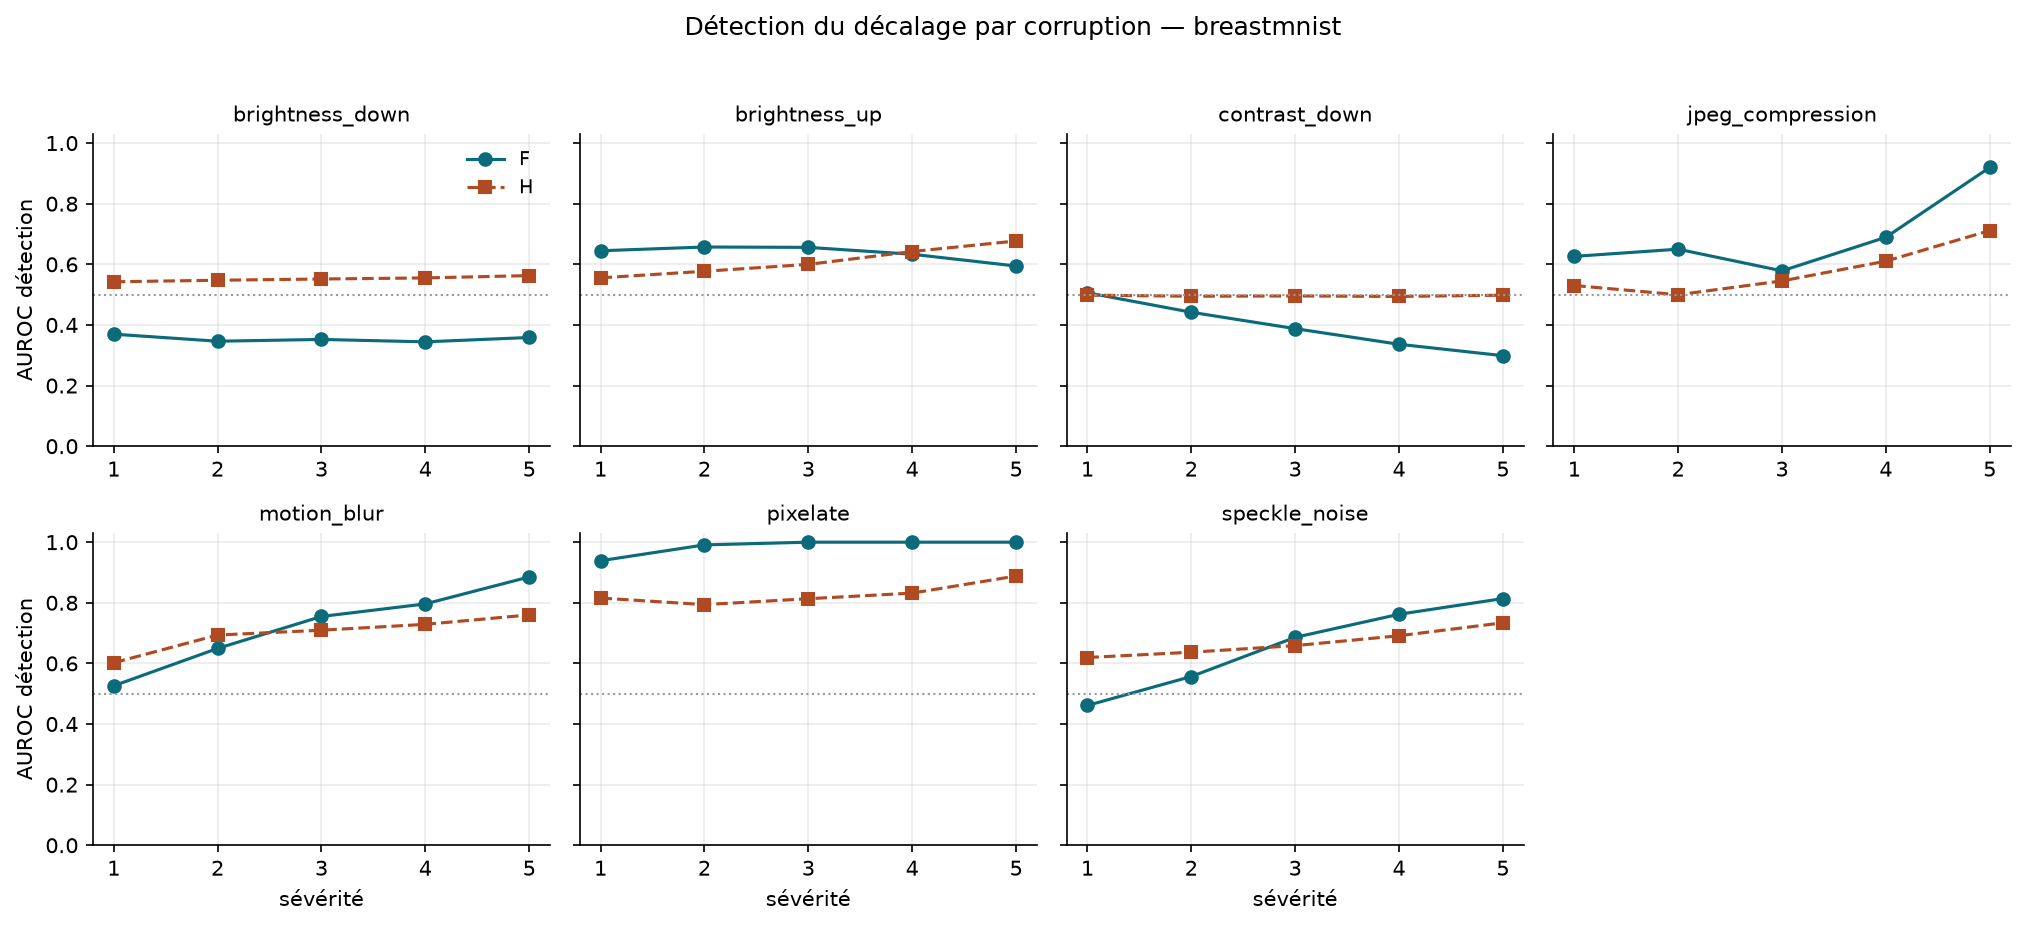
\includegraphics[width=\textwidth]{figures/fig_grid_detection_breastmnist.png}
\caption{Severity-resolved detection AUROC of $F$ (solid) and $\Hent$
(dashed) for the seven official BreastMNIST-C corruptions. Dotted line:
chance. Note the below-chance trajectories of $F$ on
\texttt{brightness\_down} and \texttt{contrast\_down}.}
\label{fig:grid}
\end{figure}

\subsection{Free energy is a signed detector}
\label{sec:signed}

The refutation has a clean geometry. On structural corruptions the corrupted
embeddings move \emph{away} from all text anchors: mean $F$ rises
monotonically with severity (BreastMNIST speckle: $1.288\!\to\!1.351$;
pixelate: $1.288\!\to\!1.479$) and $F$ dominates $\Hent$ significantly
(Table~\ref{tab:main}, upper block; all DeLong $p<0.05$, CIs excluding zero).
On photometric corruptions the embeddings move \emph{closer} to the anchors
--- mean $F$ \emph{decreases} (contrast\_down: $1.288\!\to\!1.266$;
PneumoniaMNIST gaussian\_noise: $1.264\!\to\!1.234$) --- and the one-sided
AUROC falls below $0.5$, to $0.127$ in the extreme case. A plausible reading
is that brightness/contrast compression and moderate X-ray noise push images
toward the generic, high-density region of CLIP's image manifold, reducing the
image--text modality gap; we do not claim a mechanism beyond the observed
sign.

Two practical consequences follow. First, using raw $F$ (or its negation, as
in standard energy-score OOD pipelines) as a shift alarm silently fails on
exactly the photometric drifts most typical of scanner and probe settings.
Second, the failure is directional, hence recoverable.

\subsection{A source-calibrated two-sided score rescues the inversions}
\label{sec:twosided}

The statistic $|F-\mathrm{med}_{\mathrm{src}}(F)|$ uses only source images.
At severity 5 it restores above-chance detection on five of the six
sign-inverted cases --- PneumoniaMNIST gaussian\_noise
$0.127\!\to\!0.803$, BreastMNIST contrast\_down $0.299\!\to\!0.630$,
brightness\_down $0.359\!\to\!0.606$, PneumoniaMNIST brightness\_down
$0.200\!\to\!0.598$ and contrast\_down $0.209\!\to\!0.589$ ---
while leaving structural cases essentially unchanged (pixelate $1.000$,
jpeg $0.899$, motion\_blur $0.845$, gaussian\_blur $0.962$). The recovery is
strong where the downward drift is large (X-ray Gaussian noise) and modest
where the drift is shallow relative to source dispersion (X-ray photometric
shifts, $\approx\!0.59$, where $\Hent$ itself reaches $0.64$--$0.70$).
The residual failure,
\texttt{brightness\_up} ($0.447$), is a genuinely hard case: its $F$
trajectory is non-monotonic (up at low severity, down at high), so no
function of $F$ alone can order it; its entropy signal ($0.677$) and the
X-ray photometric cases together suggest a bivariate $(F,\Hent)$ score as the
natural next step.

\begin{figure}[t]
\centering
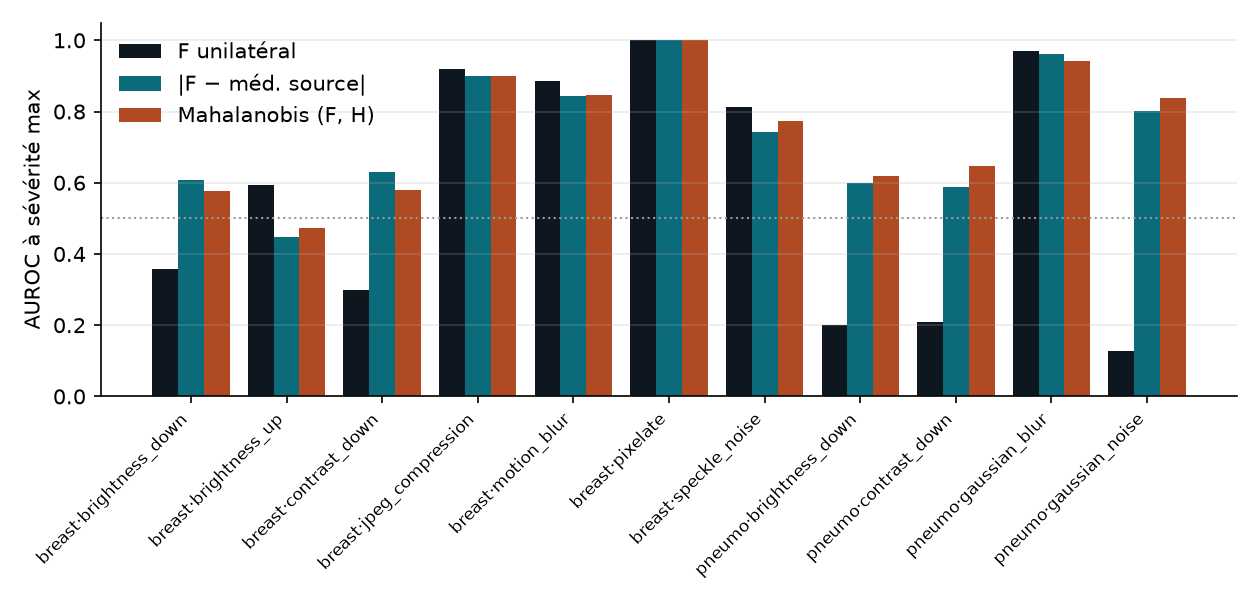
\includegraphics[width=\textwidth]{figures/fig_two_sided.png}
\caption{One-sided $F$ vs.\ two-sided $|F-\mathrm{med}_{\mathrm{src}}(F)|$
detection AUROC at maximum severity, all canonical runs.}
\label{fig:twosided}
\end{figure}

\subsection{Prompt sensitivity: $F$ is more stable than $\Hent$}
\label{sec:prompts}

The anchors are literally defined by prompt wording, so prompt sensitivity is
the substrate-specific confound. Re-running the full protocol with each single
template (BreastMNIST, severity 5):

\begin{center}
\small
\begin{tabular}{lcccc|cccc}
\toprule
 & \multicolumn{4}{c|}{AUROC($F$)} & \multicolumn{4}{c}{AUROC($\Hent$)} \\
Corruption & t0 & t1 & t2 & ens. & t0 & t1 & t2 & ens. \\
\midrule
speckle\_noise   & 0.778 & 0.801 & 0.854 & 0.814 & 0.777 & 0.641 & 0.597 & 0.734 \\
brightness\_down & 0.351 & 0.419 & 0.307 & 0.359 & 0.580 & 0.464 & 0.609 & 0.563 \\
\bottomrule
\end{tabular}
\end{center}

The dispersion of $F$ across templates (population s.d.\ over the three
isolated templates: $0.032$ on speckle, $0.046$ on brightness\_down) is roughly
half that of $\Hent$ ($0.076$ and $0.062$): the
partition function aggregates the anchor geometry and is less exposed to a
particular wording than the posterior shape. The sign inversion on
brightness\_down persists under \emph{every} template --- it is not a prompt
artifact.

\subsection{Robustness to corruption sampling}

Corruption operators are stochastic. Across three seeds (BreastMNIST,
speckle\_noise, severity 5): $\mathrm{AUROC}(F) = 0.814/0.819/0.827$,
$\mathrm{AUROC}(\Hent) = 0.734/0.749/0.738$; the paired severity-5
$\Delta$AUROC ranges $+0.069$ to $+0.088$ with overlapping CIs. Sampling noise
is an order of magnitude smaller than the effects reported above.

\subsection{Second modality}
\label{sec:pneumonia}

The chest X-ray cohort replicates the dichotomy on an independent modality,
anatomy and corruption implementation, with $4\times$ larger test sets
($n=624$). Gaussian blur (structural) behaves like the ultrasound structural
block: $F$ rises monotonically ($1.264\!\to\!1.320$) and dominates $\Hent$
($0.970$ vs.\ $0.798$, $\Delta=+0.172$, $p=4.1\times10^{-41}$). All three
photometric corruptions invert the sign of $F$ --- Gaussian noise, brightness
and contrast compression each move X-ray embeddings \emph{closer} to the text
anchors ($F$ AUROC $0.127$--$0.209$), with effect sizes far beyond sampling
noise ($|\Delta|\ge 0.335$, $p\le 10^{-86}$). On this modality the inversions
are deeper than in ultrasound, and $\Hent$ is the better detector for the two
photometric-compression cases ($0.644$ and $0.698$): neither observable
subsumes the other, which is precisely the argument for reporting both and for
the bivariate score sketched above.

\section{Discussion and limitations}
\label{sec:discussion}

\paragraph{What the refutation teaches.} The pre-registered conjecture assumed
acquisition shift acts as a quasi-uniform translation of the energy landscape.
The data say otherwise: realistic corruptions move embeddings along the
modality-gap axis in \emph{either} direction and simultaneously reshape
relative distances. The corrected picture --- $F$ as a signed coordinate of
drift along the anchor-distance axis, $\Hent$ as a shape statistic --- is more
useful than the original conjecture, and directly actionable via the two-sided
score.

\paragraph{Implications for test-time adaptation.} Entropy-minimizing TTA
\citep{wang2021tent,shu2022tpt} adapts wherever entropy is high. Our results
exhibit shifts where entropy barely moves while $F$ moves strongly (JPEG:
$\Hent$ AUROC $0.711$ vs.\ $F$ $0.920$) and shifts where entropy rises while
$F$ falls. A gating rule based on $|F-\mathrm{med}_{\mathrm{src}}|$ is the
zero-cost candidate this study puts forward for the adaptation-triggering and
early-stopping stages of our broader research program on frozen
vision--language encoders in ultrasound.

\paragraph{Limitations.} (i) Test cohorts are small ($n=156$ ultrasound
images); CIs are reported accordingly. (ii) Single backbone (CLIP ViT-B/16,
OpenAI weights); a biomedical encoder \citep{zhang2023biomedclip} may shift
the geometry and is the designated robustness check. (iii) MedMNIST-C
corruptions are synthetic surrogates for acquisition shift; the multi-center
ultrasound transfer (BUSI$\to$UDIAT$\to$BUS-UCLM) is the pre-registered next
cohort. (iv) The two-sided median is computed on the full source cohort
(in-sample); with $n=156$ and one degree of freedom the optimism is
negligible, but a held-out calibration split is the clean design. (v) Images
are $224\times224$ upsamplings of MedMNIST sources. (vi) CLIP pre-training
contamination cannot be audited (Section~\ref{sec:protocol}).

\section{Conclusion}

Under a zero-training, leakage-controlled, pre-registered protocol on official
medical corruption benchmarks, the Helmholtz free energy of a frozen CLIP
posterior is a strong but \emph{signed} detector of acquisition shift:
significantly better than entropy on structural corruptions, below chance on
photometric ones, and repaired in five of six failure cases by a two-sided
source-calibrated variant that requires nothing but source images. The strong
form of our pre-registered prediction --- entropy at chance --- is refuted and
reported as such. Every number in this paper is traceable to a versioned run;
code, metrics and raw scores are released with the paper.

\paragraph{Reproducibility.} No training anywhere; $\sim$3 minutes per
corruption sweep on CPU (156 images $\times$ 6 severities), $\sim$5 seconds on
the GPU. Each \texttt{metrics.json} records the device it ran on.
Code, per-run \texttt{metrics.json}, raw scores and analysis scripts are
available in the project repository.

\bibliographystyle{plainnat}
\bibliography{refs}

\end{document}
